\subsection{GenMAPP Builder}
\label{gmbuilder}

\subsubsection{Introduction}
\genmapp~Builder is a GUI application for loading, querying, and exporting data
used by \genmapp. The application is built from components in \emph{xmlpipedbutils} and contains the customized output from \emph{uniprotdb} and \emph{godb}. \genmapp~Builder is our final product for converting new gene sequence data from XML into \genmapp.

\subsubsection{End-Users}
\genmapp~Builder was created to be easy enough for a not-technical end user.  The interface is simple and provides access to the basic functionality required to load an XML file into a \genmapp~gene database.  \genmapp~Builder does however assume that a database administrator has prepared an accessible database server and loaded the UniProt and GO SQL database schemas.  There are four main functionalities provided by \genmapp~Builder.
\begin{itemize}
	\item {Configure the database.}
	\item {Import a UniProt XML file. }
	\item {Import a GO XML file.}
	\item {Export to \genmapp.}
\end{itemize}
The process of loading an XML file into a \genmapp~gene database starts with configuring the database connection followed by the loading of an XML file into the relational database.  The database connection must be configured to access a relational database setup by the database administrator.  Once the database connection is configured the XML files can be imported and exported without effort.  There is also an interface for HQL queries to the relational database provided by \emph{xmlpipedbutils}.  The screen shots of the application are below.

\begin{figure}[htp]
\centering
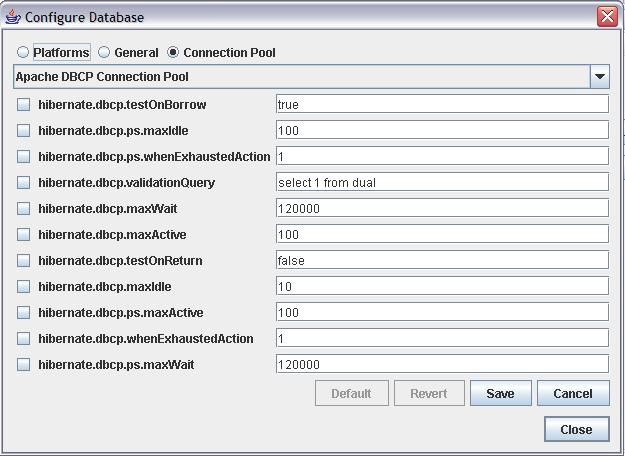
\includegraphics[scale=1.0]{Images/hibernateProps.jpg}
\caption{\small \sl The database configuration tool.}
\end{figure}

\begin{figure}[htp]
\centering
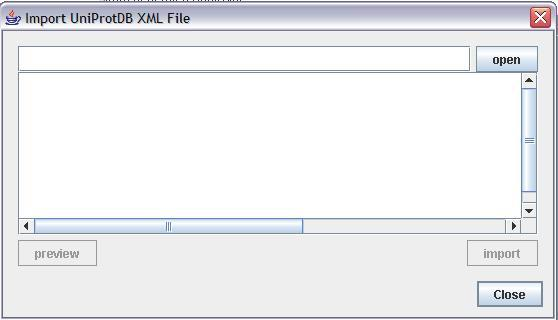
\includegraphics[scale=1.0]{Images/uniprotImport.jpg}
\caption{\small \sl The import window for UniProt XML files.}
\end{figure}

\begin{figure}[htp]
\centering
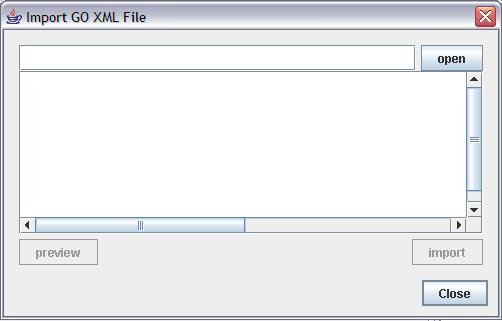
\includegraphics[scale=1.0]{Images/goImport.jpg}
\caption{\small \sl The import window for GO XML files.}
\end{figure}

\begin{figure}[htp]
\centering
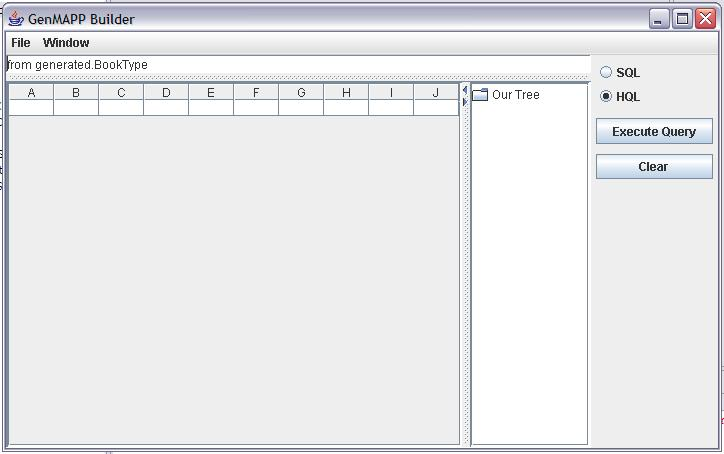
\includegraphics[scale=0.75]{Images/query.jpg}
\caption{\small \sl The relational database query interface.}
\end{figure}

\begin{figure}[htp]
\centering
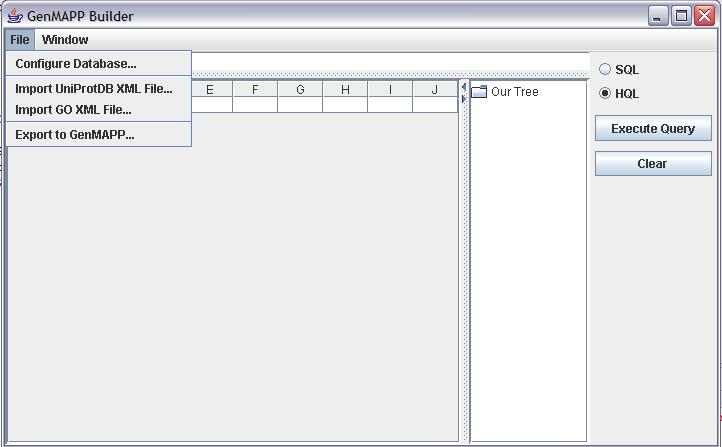
\includegraphics[scale=0.75]{Images/exportGenmapp.jpg}
\caption{\small \sl The main window with the simple drop down menu.}
\end{figure}


\subsubsection{Design}
\genmapp~Builder must create and fill the tables required in a \genmapp~gene database.  Using a template Microsoft Access (MDB) file, \genmapp~Builder fills in the system information tables: Systems, Info and Relations.  Two more stages create and fill in five more tables.

The first stage creates and fills in the Uniprot table using SQL queries.  The table is populated with the needed information extracted from the relational database. The second stage requires four GO tables to be populated with data: GeneOntology, GeneOntologyTree, GeneOntologyCount, and Uniprot-GeneOntology. At runtime, each table is created in the MDB file prior data is inserted. The following sections will discuss each table.


\paragraph{UniProt Table}
\label{uniprottable}
The UniProt table consists of entries which have an ID, name, species and date (comments and remarks are optional).  The data to populate this table comes originally from each unique entry in a given XML file.  This data must be extracted from the relational database using a pattern of SQL queries.  The extracted data is then filled into UniProt table in the MDB file.

\paragraph{GeneOntology Table}
\label{gotable}
The GeneOntology table consists of a list of GO terms, which is created by extracting all the
GO terms from the postgres database by executing HQL statements. Each term has required tags, \emph{Id} and \emph{Name}.
Each term may contain optional tags, one of which is an \emph{is\_a} tag. An \emph{is\_a} tag describes a
subclassing relationship between one term and another. Since GO terms
are organized in structures called directed acyclic graphs (DAG), each term may have many \emph{is\_a} relationships.
Terms with no \emph{is\_a} relationships are roots. Each term represents an entry in the GeneOntology table. If a term
has no \emph{is\_a} relationships, then one row is inserted into the table. If a term has one or more
\emph{is\_a} relationships, a row is inserted for each \emph{is\_a} relationships using the same term Id.


\paragraph{GeneOntologyTree Table}
The GeneOntologyTree table contains a tree representation of the GO DAG structure, which is used by MAPPFinder
to build the GO tree in the MAPPFinder browser. The algorithm that creates this table starts by inserting the root
node for each ontology. After inserting the root node, it then grabs all the children of that node and performs an insert.
For each child, it grabs its children
and performs an insert. This process continues recursively, and stops when no more child nodes exist.
Unfortunately, this table is not created from postgres, but rather from the
newly created table in Section~\ref{gotable}. The OBO.dtd file creates a SQL DDL schema which does not support
the ability to extract child nodes from a parent node. The GeneOntology table provides this functionality, which
is why it must be created first. Thus, the algorithm actually queries the MDB Access file using SQL statements.


\paragraph{GeneOntologyCount Table}
The GeneOntologyCount table contains the of number of times a GO ID appears in the GeneOntologyTree table, which
is also used by MAPPFinder to build the GO tree in the MAPPFinder browser. During the creating of the GeneOntologyTree
table, a count of each GO ID is stored in a data structure. In other words, when the algorithm grabs all child nodes from
a parent, each child node's count is increment by 1. When the GeneOntologyTree table is complete, the count for
each GO ID is extracted from the data structure and inserted into the GeneOntologyCount table.
This method was used to ``kill two birds with one stone". Otherwise,
the algorithm would have to wait until the GeneOntologyTree table was complete. Then for each GO ID, the algorithm would have
to query the GeneOntologyTree to extract the number of times it showed up in the table, which is costly and inefficient.


\paragraph{Uniprot-GeneOntology Table}
The Uniprot-GeneOntology table provides a mapping between a Uniprot ID and a GO ID, which is a many to many relationship.
Currently this information is not found in godb, but rather in an associations text file which is part of the GenMAPP Builder
resource library. Each line in the text file may contain a Uniprot ID. If it does, then there will be one to many GO ID's.
Thus, for each GO ID, a new row is created in the Uniprot-GeneOntology table with the Uniprot ID as one field and the GO ID
as another field. For example, if the line contained a Uniprot ID of \emph{00001} and three GO ID's \emph{10001,10002, and 10003},
then three row would be created with values ``00001 10001", ``00001 10002", and ``00001 10003."

\subsubsection{Performance Analysis}
\genmapp~Builder requires quite a bit of processing power and memory because of the large amount of data processed.  Initial tests of importing large XML files (40MB) took just over an hour.  Our current implementation requires a significant amount of memory because the entire file is read in as Java objects before it is pushed out to the database. Initial tests of exporting the same large XML files required nearly three hours.  Memory is not as crucial for exporting as is it for importing because only a small portion of the original data is extracted to build the \genmapp~gene database.

A couple of GO errors occurred during the first run of gmbuilder: two table fields are named \emph{Primary} and \emph{Level}, which
Microsoft Access interpreted as keywords. Additionally, the hyphen in the table \emph{Uniprot-GeneOntology}
was recognized  as a continuation line, and therefore a syntax error was generated. Fortunately, the same fix was used
in all three cases: enclose each name in double quotes. After the fix was implemented, gmbuilder successfully built the
GO tables in the MDB file, which took considerable time.

The time to build the four GO tables ran in the neighborhood of five hours (2.0GHz single processor), and
granted, this time can be shorten with better hardware. A big chunk of that time falls on the creation of the
GeneOntologyTree, although this table contains roughly seven time more entries than the table with the second
most entries. Still, it seemed that the rate of insertions per second was larger.
A good test would be to time, call it T, the creation of the
GeneOntology table by itself, then take the number of entries that were created and divide it by T. Then do the same for the
GeneOntologyTree, and compare the rate of insertions per second. If they are approximately the same, then the increased time
is due to the increase in entries. But, if the GeneOntologyTree insertion rate was much higher, than further investigation would be
needed to why the rate is slower. Perhaps it's due to the recursive nature of the algorithm, since recursion increases overhead.


\subsubsection{Future Work}
Future plans involve updating the SQL queries to HQL and creating the remaining tables that aren't part of the core table set in the MDB file. The large memory requirements could be reduced by importing the XML files into memory in portions, flushing to the database when a limit is reached. Regarding the GO tables, the algorithm that populates the GeneOntologyTree table should be investigated.
If it turns out that the GeneOntologyTree insertion rate in considerable larger that the other tables, then
a couple of solutions can be analyzed: 1) create an equivalent non-recursive function to build the tree. This
eliminates the added overhead of recursion; 2) the code can be cleaned up to
close \emph{Statement} objects before the next call to the recursive function is made. Also, the code can
be modified to use \emph{PreparedStatement} object as opposed to \emph{Statement} objects, which may be more
efficient according the java API.


As of right now, Uniprot-GeneOntology associations file is defined at a specific location in the build tree,
and the code reflects that by hardcoding the path to the file. This is error prone: every time the file changes location,
the code would also have to change, which supports poor coding practices. Also, what if the user wanted to use a different
associations file? Then the file would have to be checked in as a new resource file, and a new version of the software would have
to be released. The solution is to make this file user selectable from the genMAPP Builder GUI. This eliminate the two problems
above, while add flexibility to the user.
